\input{../../Def/defslide}
\input{../../Def/notations-hilbertfourier}
\title{MAP 555 : Analog filtering, sampling, reconstruction...}
\begin{document}
\date{18 Septembre 2015}
\maketitle



\begin{frame}
\frametitle{Today}
\tableofcontents
\end{frame}

\section{Analog filters}
\begin{frame}
\frametitle{Analog filters}
\begin{itemize}
\item The tools we have just developed (convolution and the Fourier transform for functions) are going to be used to study analog filters that are governed by a linear differential equation with constant coefficients,
$$
\sum_{k=0}^{q}b_{k}g^{(k)}=\sum_{j=0}^{p}a_{j}f^{(j)},\ a_{p}\cdot b_{q}\neq 0,
$$
where $f$ is the input and $g=A(f)$ is the output.
\item  \alert{Assumption}  $f \in \mcs(\rset)$. This case is very special. The input has no reason to be so regular, but we will see that this is a step toward more general cases.
\end{itemize}
\end{frame}

\begin{frame}
\frametitle{input and output are in $\mcs(\rset)$}
\begin{itemize}
\item Assume that $f\in \mcs(\rset)$ and look for a solution $g \in \mcs(\rset)$. If such a $g$ exists, we can take the Fourier transform of both sides of
$$
\sum_{k=0}^{q}b_{k}g^{(k)}=\sum_{j=0}^{p}a_{j}f^{(j)},\ a_{p}\cdot b_{q}\neq 0,  \quad \alert{\textbf{(S)}}
$$
showing that
$$
\sum_{k=0}^{q}b_{k}(2\rmi\pi\xi)^{k}\hat{g}(\xi)=\sum_{j=0}^{p}a_{j}(2\rmi\pi\xi)^{j}\hat{f}(\xi) \quad \alert{\textbf{(F)}}
$$
\item Consider the two polynomials $P(x)= \sum_{j=0}^{p}a_{j}x^{j}$ and $Q(x)=\sum_{k=0}^{q}b_{k}x^{k}$
and assume that the rational function $P(x)/Q(x)$ has no poles on the imaginary axis.
\end{itemize}
\end{frame}

\begin{frame}
\frametitle{input and output are in $\mcs(\rset)$}
\begin{itemize}
\item Then $P(2 \rmi\pi\xi)/Q(2 \rmi \pi\xi)$ has no poles for real $\xi$, and  \alert{\textbf{(S)}} is equivalent to
$$
\hat{g}(\xi)= G(\xi) \quad \text{where} \quad G(\xi)= \frac{P(2 \rmi \pi\xi)}{Q(2\rmi \pi\xi)}\hat{f}(\xi)
$$
Note that \alert{$G \in \mcs(\rset)$}.
\item This equality completely determines $g$ in $\mcs(\rset)$, if it exists, and thus proves the uniqueness of a solution of \alert{\textbf{(S)}} in $\mcs(\rset)$.
\item $g=\TFAC{G}$ is a solution of \alert{\textbf{(S)}} in $\mcs(\rset)$.
{\tiny The differential equation has a unique solution without initial conditions being specified. This is because we require the solution $g$ to be in $\mathcal{S}$, which means that $g$ and all of its derivatives vanish at infinity.}
\end{itemize}
\end{frame}

\begin{frame}
\frametitle{Convolution}
\begin{itemize}
\item \alert{Idea:} express the solution as a convolution.
\item \alert{Assumption:} $\deg P<\deg Q$. Define the \alert{transfer function}
$$
H(\xi)=\frac{P(2 \rmi \pi\xi)}{Q(2 \rmi \pi\xi)}
$$
is in $\ltwo(\rset) \cap \linfty(\rset)$ .
\item By decomposing this rational function into partial fractions, the \alert{impulse response}, defined as the inverse Fourier transform of the \alert{transfer function}
$$
h=\TFAC{H}
$$
is bounded, rapidly decreasing, continuous except perhaps at the origin.
\end{itemize}
\end{frame}

\begin{frame}
\frametitle{Simple poles}
\begin{itemize}
\item The poles of $P/Q$ are assumed to lie off the imaginary axis. There are two cases to consider: $P/Q$ has only simple poles or $P/Q$ has multiple poles.
\item Assume first that $P(x)/Q(x)$ has only simple poles. In this case, $H$ can be decomposed in the form
$$
H(\xi)=\sum_{k=0}^{q}\frac{\beta_{k}}{2i\pi\xi-z_{k}}
$$
where $z_{1},\ \ldots,\ z_{q}$ are the poles.
\end{itemize}
\end{frame}

\begin{frame}
\frametitle{Simple poles}
\begin{itemize}
\item For $a \in \cset$, $\mathrm{Re}(a) > 0$, $\epsilon= \pm 1$,
\[
\rme^{-\epsilon a x} u(\epsilon x) \TFyield \frac{\epsilon}{(\epsilon a + 2 \rmi \pi \xi)}
\]
\item We conclude that
$$
h(t)=\left(\sum_{k\in K-}\beta_{k} \rme^{z_{k}t} \right)u(t)- \left(\sum_{k\in K_{+}}\beta_{k} \rme^{z_{k}t} \right)u(-t) \eqsp.
$$
where $t \mapsto u(t)$ is the Heaviside function and
\begin{align*}
K_{-} &=\{k\in\{1,2,\ldots,q\}|{\rm Re}(z_{k})<0\}, \\
K_{+} &=\{k\in\{1,2,\ldots,q\}|{\rm Re}(z_{k})>0\}.
\end{align*}
\end{itemize}
\end{frame}

\begin{frame}
\frametitle{Multiple poles}
\begin{itemize}
\item Let $z_{1},\ z_{2},\ \ldots,\ z_{l}$ the poles and let $m_{1},\ m_{2},\ \ldots,\ m_{l}$ be their multiplicities.
\item Then we can write $H$ as
$$
H(\xi)=\sum_{k=1m}^{l}\sum_{=1}^{m_{k}}\frac{\beta_{k,m}}{(2i\pi\xi-z_{k})^{m}}.
$$
\item The impulse response is given by
$$
h(t)=\left(\displaystyle \sum_{k\in K-}P_{k}(t) \rme^{z_{k}t}\right)u(t)-\left(\sum_{k\in K_{+}}P_{k}(t) \rme^{z_{k}t}\right)u(-t)
$$
where
$$
P_{k}(t)=\sum_{m=1}^{m_{k}}\beta_{k,m} \frac{t^{m-1}}{(m-1)!}.
$$
\end{itemize}
\end{frame}


\begin{frame}
\frametitle{Convolution}
\begin{itemize}
\item Since $h=\TFAC{H}$ is bounded, rapidly decreasing, continuous except perhaps at the origin
\alert{\textbf{(F)}} may be rewritten as
$$
\hat{g}=\hat{h}\cdot\hat{f}.
$$
\item Since $\hat{h} \in \ltwo(\rset)$ and $\hat{f} \in \mcs(\rset) \subset \lone(\rset)$,
we have $h * f(t)= \TFAC{\hat{h} \hat{f}}$ implies that
$$
g=h*f
$$
\end{itemize}
\end{frame}

\begin{frame}
\frametitle{Generalized solutions}
The formula $g=h*f$, obtained when $f$ is in $\mathcal{S}$, makes sense in the following more general cases.
\begin{enumerate}
\item If $f$ is in $\lone(\rset)$ , then $g$ is in $\lone(\rset)\cap\ltwo(\rset)\cap \linfty(\rset)$  and
\begin{align*}
\Vert g\Vert_{1}\ &\leq\Vert h\Vert_{1}\Vert f\Vert_{1}, \\
\Vert g\Vert_{2}\ &\leq\Vert h\Vert_{2}\Vert f\Vert_{1}, \\
\Vert g\Vert_{\infty} &\leq\Vert h\Vert_{\infty}\Vert f\Vert_{1}.
\end{align*}
\item If $f$ is in $\ltwo(\rset)$ , then $g$ is in $\ltwo(\rset)$ , it is bounded and continuous, it tends to $0$ at infinity, and
\begin{align*}
\Vert g\Vert_{2}\ &\leq\Vert h\Vert_{1}\Vert f\Vert_{2}, \\
\Vert g\Vert_{\infty}& \leq \Vert h\Vert_{2}\Vert f\Vert_{2}.
\end{align*}
\item If $f$ is in $\linfty(\rset)$ , then $g$ is also bounded and
$$
\Vert g\Vert_{\infty}\leq\Vert h\Vert_{1}\Vert f\Vert_{\infty}.
$$
\end{enumerate}
\end{frame}


\begin{frame}
\frametitle{Purely imaginary poles}
\begin{itemize}
\item What we have done so far does not allow us to treat an equation like
$$
g''+\omega^{2}g=f,
$$
where $P(x)/Q(x)=1/(x^{2}+\omega^{2})$ has two poles are on the imaginary axis.
\item In this case $h$ is a sinusoid and the Fourier transform of $H$ (when $H$ is considered to be a function) is no longer defined.
\item This problem required the use of the \alert{theory of  distributions} but this degree of sophistication goes far beyond this course.
\end{itemize}
\end{frame}

\begin{frame}
\frametitle{What happens in $\deg P= \deg Q$}
Take for example the equation
$$
g''-\omega^{2}g=f''.
$$
Again, what we have done so far does not apply. Nevertheless, we can still manage to solve the equation.
Changing the unknown function to $g_0 =g-f$ lowers the order of the right-hand side:
$$
g_{0}''-\omega^{2}g_{0}=\omega^{2}f.
$$
Then we have $g_{0}=h_{0}*f$ and $g=f+h_{0}*f$.
This is \alert{no longer a convolution}  but it will serve the same purpose.
\end{frame}



\section{Linear systems}
\begin{frame}
$\Xset$ the set of \alert{input signals} and $\Yset$ the set of \alert{output signals}.\\
\alert{Assumptions}
\begin{enumerate}
\item  $\Xset$ is a vector spaces (over $\kset=\cset$ or $\kset=\rset$).
\item  $\Xset$ is closed under translation.
\end{enumerate} 
\begin{definition}[Linearity]
The system $A: \Xset \to \Yset$ is said to be \alert{linear} if for all $f_1,f_2 \in \Xset$ and $a_1,a_2 \in \kset$
$$
A(a_1 f_1 + a_2 f_2)= a_1 A(f_1) + a_2 A(f_2) \eqsp.
$$
\end{definition}
\begin{itemize}
\item \alert{A system $A$ defined $A(f) = h * f$ is linear} (assuming that $h$ and $f$ are in proper functions spaces so that $h * f$ is well defined).
\pause \begin{itemize}
\item For example, if $h \in \lone(\rset)$ then $A(f) = h * f$ is a linear system from $\Xset= \ltwo(\rset)$ onto $\Yset= \ltwo(\rset)$.
\end{itemize}
\end{itemize}

\end{frame}

\begin{frame}
\frametitle{Stability}
\begin{definition}
A system $A: \Xset \to \Yset$ is said to be \alert{stable} if there exists an $M>0$ such that $\Vert Af\Vert_{\infty}\leq M\Vert f\Vert_{\infty}$ for all $f\in \linfty(\rset)\cap \Xset$.
\end{definition}
\begin{enumerate}
\item The generalized filter $A$ is stable when $\deg P<\deg Q$.
\item It is still stable if $\deg P = \deg Q$...
\item Set $\Xset=\Yset=\ltwo(\rset)$ and $h \in \lone \rset$. Then $A(f)= h * f$, with $f \in \ltwo(\rset)$ is stable.
 \end{enumerate}
\end{frame}

\begin{frame}
\frametitle{Causality}
\begin{definition}
A system $A: \Xset \to \Yset$ is \alert{causal} if the equality of any two input signals up to time $t=t_0$ implies the equality of the two output signals at least to time $t_0$,
$$
\text{$f_1(t)= f_2(t)$ for $t \leq t_0$} \Rightarrow \text{$A f_1(t)= A f_2(t)$ for $t < t_0$}
$$
\end{definition}
This property is completely natural for a physical system in which the
variable is time. It says that the response at time $t$ depends only on what
has happened before $t$.
\end{frame}

\begin{frame}
\frametitle{Causality}
\begin{theorem}
If $A(f)= h * f$ is a defined with a convolution, then the system is causal if the impulse response vanishes for all $x \leq 0$.
\end{theorem}
\begin{itemize}
\item The system $A(f)= h * f$ with $h(x)= u(x) \rme^{-a x}$ $a > 0$ is causal (since $h \in \lone(\rset)$, we may take here $\Xset= \Yset= \ltwo(\rset)$). The support of the impulse reponse is $\rset^+$ (it is infinite).
\item more generally, if  $\deg P < \deg Q$, the generalized filter $A: A(f)= h * f$ is \alert{causal} if $\supp(h) \subset \coint{0,\infty}$ or equivalently if the poles of $P/Q$ are located to the \alert{left of the imaginary axis}.
\end{itemize}
\end{frame}

\begin{frame}
\frametitle{Invariance}
Define by $\tau_a$ the \alert{delay operator}: $\tau_a f(x)= f(x-a)$ for all $x \in \rset$.
\begin{definition}
A system $A$ is \alert{invariant} if a translation of time in the input leads to the same translation in the output, or equivalently
if $A$ and $\tau_a$ commute for all $a \in \rset$:
\[
A \circ \tau_a = \tau_a \circ A
\]
\end{definition}
\begin{itemize}
\item if $\Xset= \Yset= \ltwo(\rset)$, $h \in \lone(\rset)$, then $A(f)= h * f$ is invariant. 
\end{itemize}
\end{frame}

\begin{frame}
\frametitle{Linear filter}
\begin{definition}
A mapping $A: \Xset \to \Yset$ is a \alert{linear filter} if 
\begin{enumerate}
\item $A$ is linear 
\item $A$ is invariant. 
\end{enumerate}
\end{definition}
\begin{itemize}
\item $\Xset= \Yset= \ltwo(\rset)$, $h \in \lone(\rset)$, $A(f)= h * f$ is a linear filter.
\item If $\Xset \subset C^1(\rset)$ is the set of functions $f$ satisfying $f(x)= \int \hat{f}(\xi) \rme^{+ 2 \rmi \pi \xi x} \rmd \xi$ for all $x \in \Xset$ for some $(1 + \|\xi|) \hat{f} \in \lone(\rset)$. The mapping $A(f)= f'$ is a linear filter. Its transfer function is $H(\xi)= 2 \rmi \pi \xi$ but this is not a \alert{convolution}.
\end{itemize}
\end{frame}

\begin{frame}
\frametitle{A first order filter}
\begin{itemize}
\item Consider the first order system $RC g' + g = f$. 
\item This is rational system with $P(x)= 1$ and $Q(x)= 1 + RC(x)$ ($\mathrm{deg}(P) < \mathrm{deg}(Q)$)
\item The \alert{transfer function} is 
\[
H(\xi)= \frac{P(2 \rmi \pi \xi)}{Q(2 \rmi \pi \xi)}= \frac{1}{1 + 2 \rmi RC \pi \xi }
\]
There is a \alert{single pole} at $z_1= -1/RC$. The system is \alert{low pass}.
\item The \alert{impulse response} is 
\[
h(t)= \frac{1}{RC} \rme^{-t/RC} u(t) \eqsp.
\] 
\item This is a convolutive system, which is causal and stable, which may be defined on $\Xset = \ltwo(\rset)$ by
\[
g= A(f)= \int h(s) f(t-s) \rmd s \eqsp.
\]
\end{itemize}
\end{frame}
\section{Sampling}
\begin{frame}
\frametitle{Periodic sampling ?}
\begin{figure}
  \centering
  % Requires \usepackage{graphicx}
  \includegraphics[width=0.6\textwidth]{sampling}\\
\end{figure}
\alert{$T$} the \alert{sampling period}. \alert{$f[n]= f(nT)$} are the samples of the signals.
The \alert{sampling frequency} \alert{$1/T$}.
\end{frame}


\begin{frame}
\frametitle{Band Limited functions}
\begin{definition}[Band Limited function]
A function $f \in L_2(\rset)$ is said to be  \alert{band limited} if there exists $B < \infty$ such that: $\TF f(\xi) = 0$ pour $\xi \not \in [-B,+B]$. We denote $\BL{B}$ the subspace of $f \in L_2(\rset)$ of functions satisfying $\TF f(\xi) = 0$ for (almost) all $\xi \not \in [-B,+B]$.
\end{definition}
\end{frame}

\begin{frame}
\frametitle{Band-Limited functions}
\begin{itemize}
\item The Fourier transform defines an isomporphism on $L_2(\rset)$. The inverse is $\TFC$.
\item Let  $f \in \BL{B}$. Since $\TF f$ is compactly supported and belongs $L_2(\rset)$, $\TF f  \in \lone(\rset)$.
\item Therefore $x \mapsto \TFC \circ \TF f(x)$ is continuous and since $\TFC \circ \TF f= f$ a.e., every function in $\BL{B}$ has a continuous version (and even a $C^\infty$ version).
\end{itemize}
\end{frame}

\begin{frame}
\frametitle{Periodizing the Fourier transform}
\only<1->{Let $T \leq 1/(2B)$ be the \alert{sampling period} and $1/T$ be the \alert{sampling frequency}.
Consider the periodic function $\xi \to \TF f(\xi)$ given by:
$$
F_T (\xi) = \sum_{n \in \zset} [\TF f] \left( \xi - \frac{n}{T} \right) \eqsp.
$$
}
\only<2>{$\xi \mapsto F_T(\xi)$ is periodic with period $1/T$}
\only<3>{The function  $F_T \in L_2{[-1/2T,1/2T]}$ can be expanded as a series function
\begin{equation*}
F_T (\xi) = \sum_{n \in \zset} c_n(F_T) \rme^{- \rmi 2 \pi \xi n T},
\end{equation*}
where $\{c_k(F_T)\}$, the Fourier coefficients are given by
\begin{equation*}
c_k(F_T) = T \int_{-1/(2T)}^{1/(2T)} F_T(\xi) \rme^{+ \rmi 2 \pi \xi k T} \rmd \xi\eqsp.
\end{equation*}
}
\end{frame}

\begin{frame}
\frametitle{Periodizing the Fourier transform}
The identity
\begin{equation*}
F_T (\xi) = \sum_{n \in \zset} c_n(F_T) \rme^{- \rmi 2 \pi \xi n T},
\end{equation*}
should be understood as a convergence of the partial sums
\begin{equation*}
F_{N,T}(\xi)= \sum_{k=-N}^N c_N(F_T) \rme^{- \rmi 2 \pi \xi n T} \eqsp,
\end{equation*}
toward $F_T$ in the topology induced by the norm $\|\cdot\|_2$  in $L_2([-1/(2T),1/(2T)])$:
$$
\lim_{N \to \infty} \int_{-1/(2T)}^{1/(2T)} |F_T(\xi) - F_{N,T}(\xi)|^2 \rmd \xi =0 \eqsp.
$$
\only<2>{The Parseval identity implies that $\sum_{n \in \zset} |c_n(F_T)|^2 < \infty$}.
\end{frame}

\begin{frame}
\frametitle{A key result}
\begin{itemize}
\item Since for all $T \leq 1/(2B)$, $[-B,+B] \subset [-1/(2T), 1/(2T)]$, then for all $\xi \in [-1/(2T),1/(2T)]$,
\alert{
$$F_T(\xi) = \TF f(\xi) $$
}
\item Therefore, the  Fourier coefficients $c_k(F_T)$ are given by:
\alert{
\begin{equation*}
c_k(F_T) = T \int_{-B}^{B} \TF f(\xi) \rme^{+ \rmi 2 \pi \xi k T} \rmd \xi= T f(kT)\eqsp.
\end{equation*}
}
\end{itemize}
\end{frame}



\begin{frame}
\frametitle{The Poisson Formula: Key result}
If $f \in \BL{B}$ then the \alert{discrete-time Fourier transform} (DTFT) of the sequence of samples $\{ f(nT), n \in \zset \}$
\[
T \sum_{n \in \zset} f(nT) \rme^{- \rmi 2 \pi \xi n T}
\]
is equal to the Fourier transform of the function $f$ periodized with a period $1/T$, a relation called the \alert{Poisson formula}
\begin{equation*}
\label{eq:FormuleSommatoirePoisson}
\sum_{n \in \zset} \TF f \left( \xi - \frac{n}{T} \right)  = T \sum_{n \in \zset} f(nT) \rme^{- \rmi 2 \pi \xi n T}\eqsp,
\end{equation*}
\only<2>{An amazing result: the DTFT is computable only from the knowledge of the samples $\{x(nT), n \in \zset\}$, whereas
the knowledge of $\TF f$ requires to evaluate the function at all time points
}
\only<3>{the DTFT is periodic with period $1/T$, which is the sampling frequency. Because of this periodicity, one may restrict the frequency
interval to just one-period, $[-1/2T,1/2T]$}
\end{frame}

\begin{frame}
\frametitle{Interpolation formula}
\begin{itemize}
\item \alert<1>{Multiply the Poisson formula
\begin{equation*}
\sum_{n \in \zset} \TF f \left( \xi - \frac{n}{T} \right)  = T \sum_{n \in \zset} f(nT) \rme^{- \rmi 2 \pi \xi n T}\eqsp,
\end{equation*}
by the indicator function $\1_{[-1/(2T),1/(2T)]}(\xi)$}
\item \alert<2>{Use the identity $$\1_{[-1/(2T),1/(2T)]}(\xi) \TF f (\xi)= \1_{[-1/(2T),1/(2T)]}(\xi) F_T(\xi)$$}
\end{itemize}

\end{frame}

\begin{frame}
\frametitle{Interpolation formula}
For all $\xi \in [-1/2T,+1/2T]$,
$$
\TF f (\xi) = T \sum_{n \in \zset} f(nT) \1_{[-1/(2T),1/(2T)]}(\xi) \rme^{- \rmi 2 \pi \xi n T} \eqsp.
$$
which should be understood as
$$
\lim_{N \to \infty} \int \left| \TF f(\xi)  - T \sum_{n =-N}^N f(nT) \1_{\left[-\frac{1}{2T},\frac{1}{2T}\right]}(\xi) \rme^{- \rmi 2 \pi
    \xi n T}  \right|^2 \rmd \xi = 0 \eqsp.
$$
Since $\TFC$ is an isometry and $\TFC \TF f = f$ a.e.
$$
\lim_{N \to \infty} \int \left| f(t)  - T \sum_{n =-N}^N f(nT) \TFAC{\1_{\left[-\frac{1}{2T},\frac{1}{2T}\right]}(\xi) \rme^{+ \rmi 2 \pi
    \xi n T}}(t) \right|^2 \rmd t = 0 \eqsp.
$$
\end{frame}

\begin{frame}
\frametitle{Interpolation formula}
\begin{lemma}
$$
\TFAC{\xi \to \1_{[-1/(2T),1/(2T)]}(\xi) \rme^{+ \rmi 2 \pi \xi n T}}(x)= \frac{\sin\left( \frac{\pi}{T}(x - nT)\right)}{\pi(x-nT)}
$$
\end{lemma}


\end{frame}

\begin{frame}
\frametitle{Interpolation formula}
\begin{theorem}[Nyquist theorem]
If $f \in \BL{B}$ and $T \leq 1/2B$ then
\alert{
\begin{equation*}
f(x) =_{\ltwo(\rset)} \sum_{n \in \zset} f(nT) s_T(x-nT)  \eqsp,
\end{equation*}
}
where $s_T$, is the cardinal-sine function
\alert{
$$
s_T(x) = \frac{\sin \left( \pi x/T\right) }{ \pi x/T}\eqsp.
$$
}
If in addition,
$$
\sum_{k \in \zset} |f(kT)| < \infty,
$$
the series converges uniformly to $f$.
\end{theorem}
The condition  \alert{$T \leq 1/2B$} is the \alert{Nyquist condition}.
\end{frame}

\section{Aliasing}
\begin{frame}
\frametitle{What happens if the Nyquist condition is violated ?}
\begin{itemize}
\item Assume that $f \in \BL{B}$ but $T \geq 1/(2B)$.
\item It still makes sense to consider the periodization of the Fourier transform
$$
F_T (\xi) = \sum_{n \in \zset} [\TF f] \left( \xi - \frac{n}{T} \right) \eqsp.
$$
\item \alert<2>{but now the different spectral replicas now overlap, a phenomenon called aliasing.}
\end{itemize}
\end{frame}

\begin{frame}
\frametitle{Aliasing}
\begin{itemize}
\item The periodized spectrum $\xi \mapsto F_T(\xi)$ still belongs to $L^2(\rset)$.
\item We may still develop this function as a Fourier series:
\begin{equation*}
F_T (\xi) =  \sum_{n \in \zset} c_k(T) \rme^{- \rmi 2 \pi \xi n T},
\end{equation*}
where $c_k(T)$ are the Fourier coefficients.
\item \alert{Key result !} We still have
\[
c_k(T)= T f(kT)
\]
the Fourier coefficients of the periodized spectrum are the samples of the functions !
\end{itemize}
\end{frame}

\begin{frame}
\frametitle{Aliasing...}
The Fourier transform of the Nyquist interpolation
\begin{equation*}
\tilde{f}(x) = \sum_{n \in \zset} f(nT) s_T(x-nT)  \eqsp,
\end{equation*}
is the $\BL{1/2T}$ function whose Fourier transform is equal to
\[
\1_{[-1/2T,1/2T]}(\xi) \sum_{n=-\infty}^{\infty} \TF f(\xi - n/T)
\]
\only<2>{\alert{Beware !} It is essential to use a lowpass antialiasing prefilter to bandlimit the input signal to within the
\alert{Nyquist interval} so that the resulting replicas after sampling will not overlap}
\end{frame}

\begin{frame}
\frametitle{An illustration}
\begin{itemize}
\item This example illustrates the effect of sampling a non bandlimited signal and the degree to which the portion of the Fourier transform (\alert{spectrum}) within the Nyquist interval approximates the original spectrum.
\item Consider the exponentially decaying signal and its spectrum
\[
f(x) = \rme^{-a x} u(x) \eqsp, \quad \TF f(\xi)= \frac{1}{a + 2 \pi \rmi \xi} \eqsp.
\]
\item The discrete time Fourier transform of the sampled signal can be obtained in two different ways...
\end{itemize}
\end{frame}


\begin{frame}
\frametitle{Calculation of the DFT}
\begin{align*}
\hat{F}_T(\xi)
&= T \sum_{n=-\infty}^{\infty} f(nT) \rme^{- \rmi 2 \pi n \xi T}  \\
&= T \sum_{n=0}^\infty \rme^{-a n T} \rme^{- \rmi 2 \pi n \xi T} = \frac{T}{1-\rme^{-aT} \rme^{-\rmi 2 \pi \xi T}}
\end{align*}
On the other hand, by the Poisson formula (which is still valid) the DTFT is the equal to the periodized spectrum
\[
\hat{F}_T(\xi) = \sum_{m=-\infty}^{\infty} \frac{1}{a + 2 \pi \rmi (\xi - n \xi_s)}
\]
where $\xi_s= 1/T$ is the \alert{sampling frequency}.

\end{frame}

\begin{frame}
\frametitle{A not so-obvious identity}
\begin{itemize}
\item Combining the two expressions of the DTFT, we obtain the not-so-obvious identity
\[
\sum_{m=-\infty}^{\infty} \frac{1}{a + 2 \pi \rmi (\xi - n \xi_s)} = \frac{T}{1-\rme^{-aT} \rme^{-\rmi 2 \pi \xi T}}
\]
\item  \alert{A sanity check}... When $T \to 0$ (the sampling frequency goes to $\infty$), then
\[
\frac{T}{1-\rme^{-aT} \rme^{-\rmi 2 \pi \xi T}} \to \frac{1}{a + 2 \pi \rmi \xi}
\]
\end{itemize}
\end{frame}

\begin{frame}
\frametitle{Aliasing: the exponential case}
\begin{figure}
  \centering
  % Requires \usepackage{graphicx}
  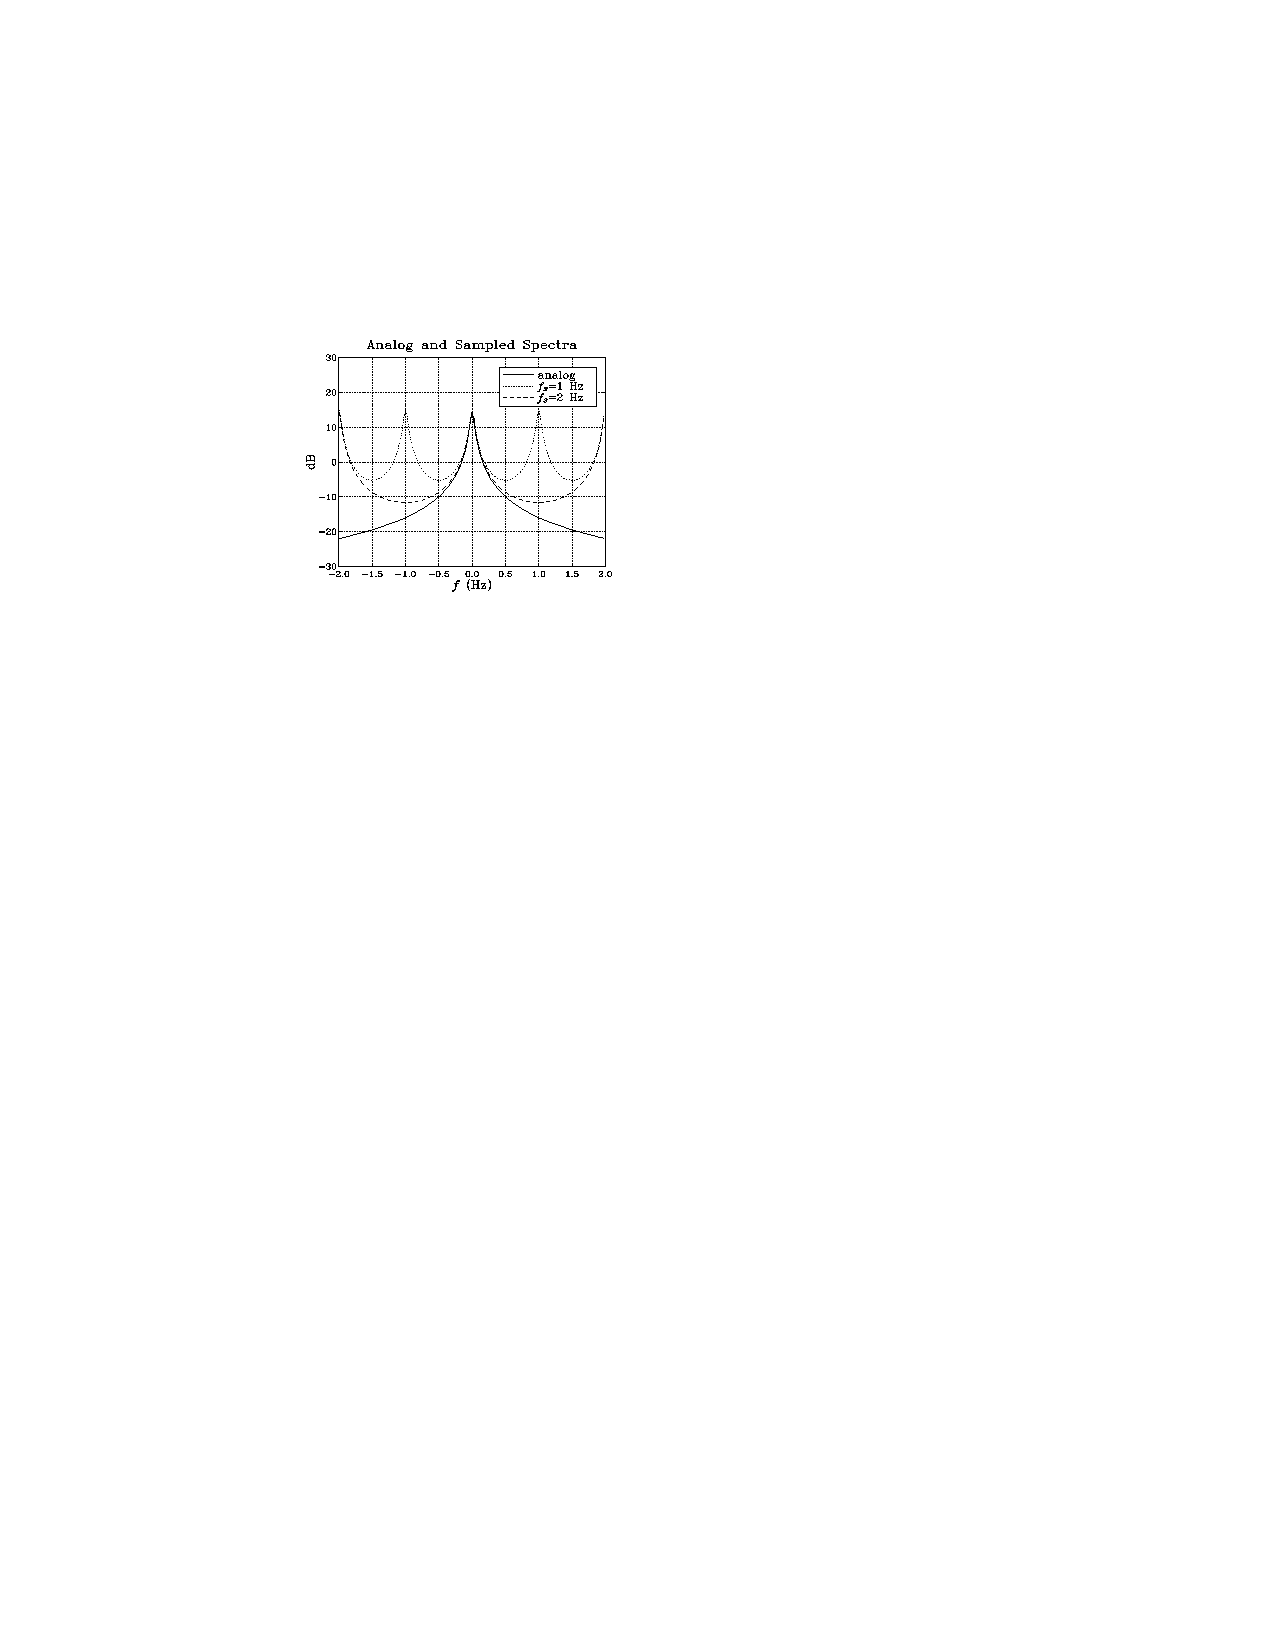
\includegraphics[width=0.8\textwidth]{aliasing-expo}\\
\end{figure}
\end{frame}

\begin{frame}
\frametitle{Ideal antialiasing filter}

\begin{figure}
  \centering
  % Requires \usepackage{graphicx}
  \includegraphics[width=0.8\textwidth]{IdelaAntiAlias}\\
  \caption{An ideal analog lowpass prefilter removes all the frequency components of the analog input that lie beyond the Nyquist frequency $\xi_s/2$}
\end{figure}


\end{frame}

\begin{frame}
\frametitle{Practical antialiasing filter}
\begin{itemize}
\item Antialiasing filter used in practice are not ideal and do not completely remove all the frequency components outside the Nyquist interval. Thus, some \alert{aliasing will always take place}.
\item By proper design, the prefilters may be made as good as desired and the amount of aliasing reduced to tolerable levels.
\item A practical anti-aliasing filter is a low pass filter with passband usually taken to be the \alert{frequency-range of interest} for the application at hand and \alert{must be entirely within the Nyquist interval}.
\end{itemize}
\end{frame}

\begin{frame}
\frametitle{Practical antialiasing filter}

\begin{figure}
  \centering
  % Requires \usepackage{graphicx}
  \includegraphics[width=0.6\textwidth]{PracticalAntiAlias}\\
  \caption{Practical antialiasing lowpass filter}
\end{figure}

\end{frame}

\begin{frame}
\frametitle{Practical antialiasing filter}
\begin{itemize}
\item The prefilter must be essentially flat over his passband in order not to distort the frequencies of interest.
\item Even if it is not completely flat over the passband, it can be \alert{equalized} digitally at a subsequent processing stage by a \alert{digital filter}.
\item The \alert{stopband frequency} $\xi_{\mathrm{stop}}$ of the prefilter and the \alert{minimum stop band attenuation} must be chosen appropriately to minimize aliasing effects.
\item The stop band frequency should be chosen so that
\[
\xi_{\mathrm{stop}}= \xi_{\mathrm{s}} - \xi_{\mathrm{pass}} \eqsp.
\]
\end{itemize}
\end{frame}

\section{Practical reconstruction}
\begin{frame}
\frametitle{Analog reconstructors}
\begin{itemize}
\item The ideal interpolation is not physically achievable (the support of $s_T$ is the whole real-line and is non causal).
\item Any reasonable way of \alert{filling the gaps} between samples will result in some sort of reconstruction.
\item A typical reconstruction formula is
\alert{
\[
f_a(x)= \sum_{n=-\infty}^\infty f(nT) h_T(x-nT)
\]
}
where $h_T$ has a \alert{finite support}.
\item The simplest reconstruction formula is the \alert{sample and hold} or \alert{staircase} in which $h_T(x)= \1_{[0,T]}(x)$.
\end{itemize}
\end{frame}

\begin{frame}
\frametitle{Staircase reconstructor}
\begin{figure}
  \centering
  % Requires \usepackage{graphicx}
  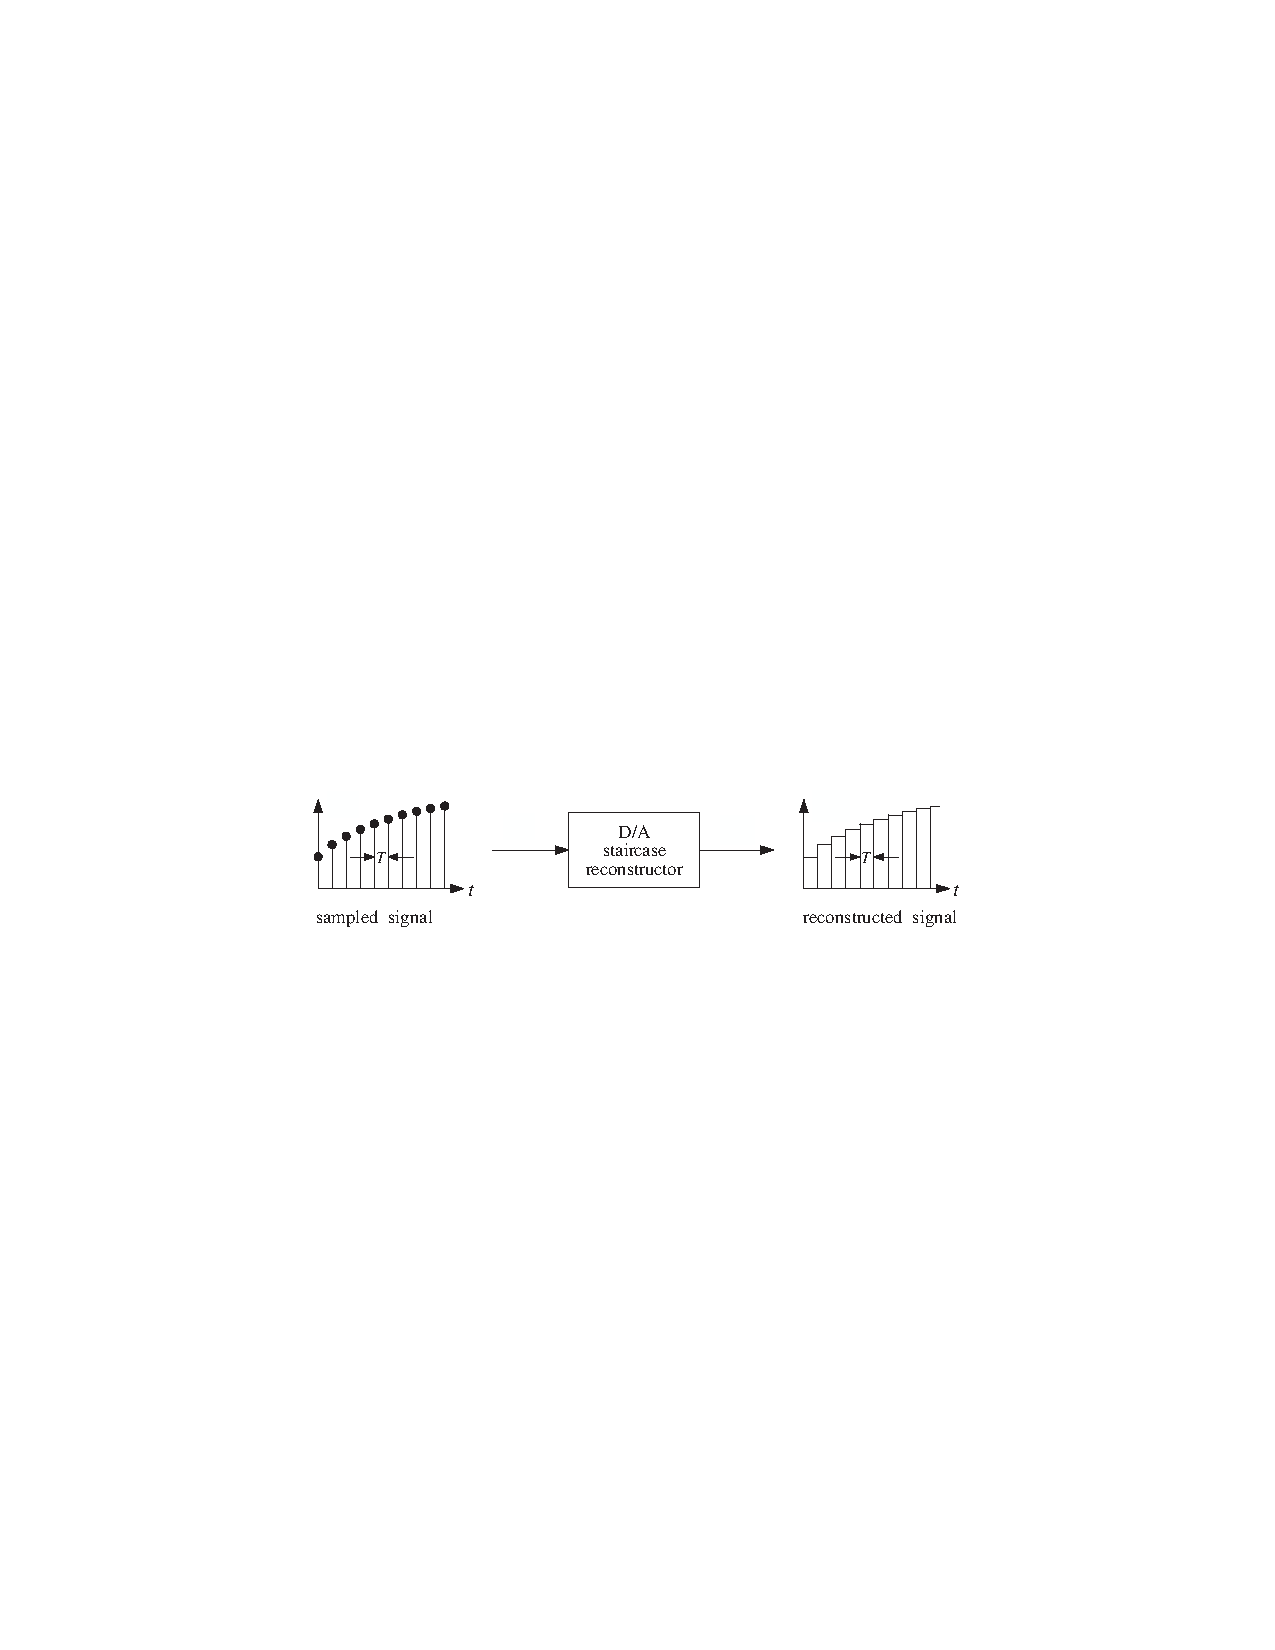
\includegraphics[width=0.9\textwidth]{staircase}\\
\end{figure}

\end{frame}

\begin{frame}
\frametitle{Practical reconstructor}
\begin{itemize}
\item Assume that $h_T \in \lone(\rset) \times \ltwo(\rset)$. Then
$$
\TF h_T (\xi)= \hat{h}_T(\xi)= \int_{-\infty}^\infty h_T(x) \rme^{-\rmi 2 \pi \xi x} \rmd x
$$
Note that $\hat{h}_T \in \ltwo(\rset) \cap \linfty(\rset)$.
\item For any $N \in \nset$,
\begin{align*}
\TFAC{\sum_{n=-N}^{N} f(nT) h_T(x - nT)}(\xi)
&= \hat{h}_T(\xi) \sum_{n=-N}^N f(nT) \rme^{-\rmi 2 \pi \xi nT} \\
&= T^{-1} \hat{h}_T(\xi) \alert{F_{N,T}(\xi)}
\end{align*}
\end{itemize}

\end{frame}

\begin{frame}
\frametitle{Practical reconstruction}
\begin{itemize}
\item $\lim_{N \to \infty} \| F_{N,T} - F_T \|_2= 0$ where $F_T$ is the $T$-periodized spectrum.
\item Therefore, in $\ltwo(\rset)$,
\alert{\begin{multline*}
\TFAC{\sum_{n=-N}^{N} f(nT) h_T(x - nT)}(\xi) \\
= T^{-1} \hat{h}_T(\xi) \sum_{m=-\infty}^\infty \TF f(\xi -  m/T)
\end{multline*}}
\only<2>{\item \alert{Practical interpolators do not completely eliminate the replicated spectral images as the ideal reconstructor does.}}
\end{itemize}

\end{frame}

\begin{frame}
\frametitle{Staircase reconstruction}
For the staircase reconstructor, $h_T(x) = \1_{[0,T]}(x)$ and
\[
\hat{h}_T(\xi)= T \frac{\sin(\pi \xi T)}{\pi \xi T} \rme^{-\rmi \pi \xi T} \eqsp.
\]
\begin{figure}
  \centering
  % Requires \usepackage{graphicx}
  \includegraphics[width=0.5\textwidth]{staircasefourier}
\end{figure}
\end{frame}

\begin{frame}
\begin{figure}
  \centering
  % Requires \usepackage{graphicx}
  \includegraphics[width=0.7\textwidth]{staircasespectrum}
  \caption{The staircase reconstructor does not completely eliminate the replicated spectral images as the ideal reconstructor does}
\end{figure}
\end{frame}

\begin{frame}
\frametitle{Anti-image postfilters}
\begin{itemize}
\item The surviving spectral replicas may be removed by an additional \alert{lowpass filter}, called the \alert{anti-image postfilter},
whose cutoff frequency in the Nyquist frequency $\xi_s/2$.
\item In the frequency domain, the combined effect of the staircase reconstructor followed by the anti-image postfilter is to remove the spectral replica as much as possible.
\item The reason for using this two-stage reconstruction procedure is the \alert{simplicity} pf implementation of the staircase reconstruction. A typical D/A converter will act as such a reconstructor.
\end{itemize}
\end{frame}

\begin{frame}
\frametitle{Anti-image postfilters}
\begin{figure}
  \centering
  % Requires \usepackage{graphicx}
  \includegraphics[width=0.9\textwidth]{antiimagepost}\\
\end{figure}
\end{frame}

\section{Another approach to sampling}
\begin{frame}
\frametitle{Why ?}
\begin{itemize}
\item Sampling theorem can be derived from another perspective, which is in some sense broader.
\item It acknowledges the fact that a function can be seen as a superposition if complex exponential (\alert{think !} this is the meaning of the Fourier synthesis formula...)
\item The approach starts by deriving the sampling theorem first for complex exponential, and then to extends the result to a (much) wider class of signals.    
\end{itemize}
\end{frame}

\begin{frame}
\frametitle{Problem}
\begin{itemize}
\item Consider the function $s_{\xi_0}(x)= \rme^{2 \rmi \pi \xi_0 x}$, $\xi_0 \in \rset$. This function is neither in $\lone(\rset)$ or in $\ltwo(\rset)$, and therefore does not fit into the framework presented earlier.
\item A natural question is the following: under which conditions on the sampling period $T$ may we retrieve $s(x)$ from the its samples $\{s(nT), n \in \zset\}$.
\item Since $s_{\xi_0}(nT)= \rme^{2 \rmi \pi \xi_0 n T}$, we have 
$$
s_{\xi_0}(nT)= s_{\xi_0 + k/T}(nT) \eqsp, \quad \text{for all $k,n \in \zset$}
$$ 
\item If $\xi_0 \in \ooint{-1/2T,1/2T}$ we can retrieve $s_{\xi_0}$ from its samples without error !
\end{itemize}
\end{frame}


\begin{frame}
\frametitle{A sampling theorem for complex exponential}
\begin{theorem}
For all $x \in \rset$ and  $\xi_0 \in \ooint{-1/2T,1/2T}$,
\[
\rme^{2 \rmi \pi \xi_0 x} = \sum_{n \in \zset} \rme^{2 \rmi \pi \xi_0 n T} s_T(x - nT) \quad s_T(x)= \frac{\sin\left( \pi x/T \right)}{\pi x /T}
\]
where the series in the RHS converges uniformly on $\ccint{-B,B} \subset \ooint{-1/2T,1/2T}$
\end{theorem}
\end{frame}

\frame[plain]{\includegraphics[width=\textwidth]{interpolation-sinewave}}

\begin{frame}
\frametitle{Sampling a decomposable signal}
\begin{itemize}
\item If $x \mapsto f(x)$ is a finite superposition of complex sinewaves, 
\[
f(x)= \sum_{k=1}^M \gamma_k \rme^{2 \rmi \nu_k x}
\]
where $\{\gamma_k\}_{k=1}^M \in \cset$ and $\{ \nu_k \}_{k=1}^M \subset \ooint{-1/2T,1/2T}$, then the Nyquist formula holds
\[
f(x)= \sum_{k=-\infty}^{\infty}  f(kT) s_T(x - kT)
\]
\item This can be extended to any function $f$ which can be written as
\[
f(x)= \int_{-B}^B \rme^{2 \rmi \pi \xi x} \mu(\rmd x)
\]
where $\mu$ is a measure on $\ccint{-B,B}$ as soon as $B < 1/2T$.
\end{itemize}
\end{frame}

\end{document} 